\documentclass[tikz]{standalone}

\usetikzlibrary{shapes}

\begin{document}

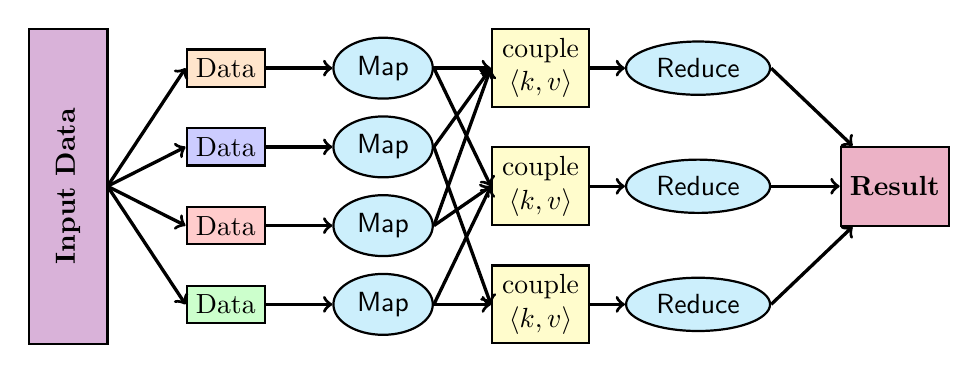
\begin{tikzpicture}[every node/.style={thick}]
  \colorlet{coul0}{orange!20} \colorlet{coul1}{blue!20} \colorlet{coul2}{red!20} \colorlet{coul3}{green!20}
  \tikzstyle{edge}=[->, very thick]
  \draw[thick, fill=violet!30] (-1, -2) rectangle node[rotate=90] {\textbf{Input Data}} (0,2);
  \foreach \i in {0,1,2,3} {
    \node[draw, fill=coul\i] (data\i) at (1.5, 1.5 - \i) {Data};
    \node[ellipse, draw, fill=cyan!20] (map\i) at (3.5, 1.5 - \i) {\textsf{Map}};
    \draw[edge] (0,0) -- (data\i.west);
    \draw[edge] (data\i) -- (map\i);
  }
  \node[draw, minimum height=1cm, fill=purple!30] (resultat) at (10, 0) {\textbf{Result}};
  \foreach \i in {0,1,2} {
    \node[draw, fill=yellow!20] (paire\i) at (5.5, 1.5 - \i*1.5) {\begin{minipage}{1cm}couple \centering $\langle k,v \rangle$\end{minipage}};
    \node[ellipse, draw, fill=cyan!20] (reduce\i) at (7.5, 1.5 - \i*1.5) {\textsf{Reduce}};
    \draw[edge] (paire\i) -- (reduce\i);
    \draw[edge] (reduce\i.east) -- (resultat);
  }
          %paire
  \draw[edge] (map0.east) -- (paire0.west); \draw[edge] (map0.east) -- (paire1.west);
  \draw[edge] (map1.east) -- (paire0.west); \draw[edge] (map1.east) -- (paire2.west);
  \draw[edge] (map2.east) -- (paire1.west); \draw[edge] (map2.east) -- (paire0.west);
  \draw[edge] (map3.east) -- (paire1.west); \draw[edge] (map3.east) -- (paire2.west);
\end{tikzpicture}

\end{document}